% Graphic for TeX using PGF
% Title: C:\Users\CAMUGLIAL_INFO\Desktop\Diplome\Diplome\_Documentation\Diagrammes\Inscription.dia
% Creator: Dia v0.97.2
% CreationDate: Fri May 26 08:34:49 2017
% For: admintech
% \usepackage{tikz}
% The following commands are not supported in PSTricks at present
% We define them conditionally, so when they are implemented,
% this pgf file will use them.
\ifx\du\undefined
  \newlength{\du}
\fi
\setlength{\du}{15\unitlength}
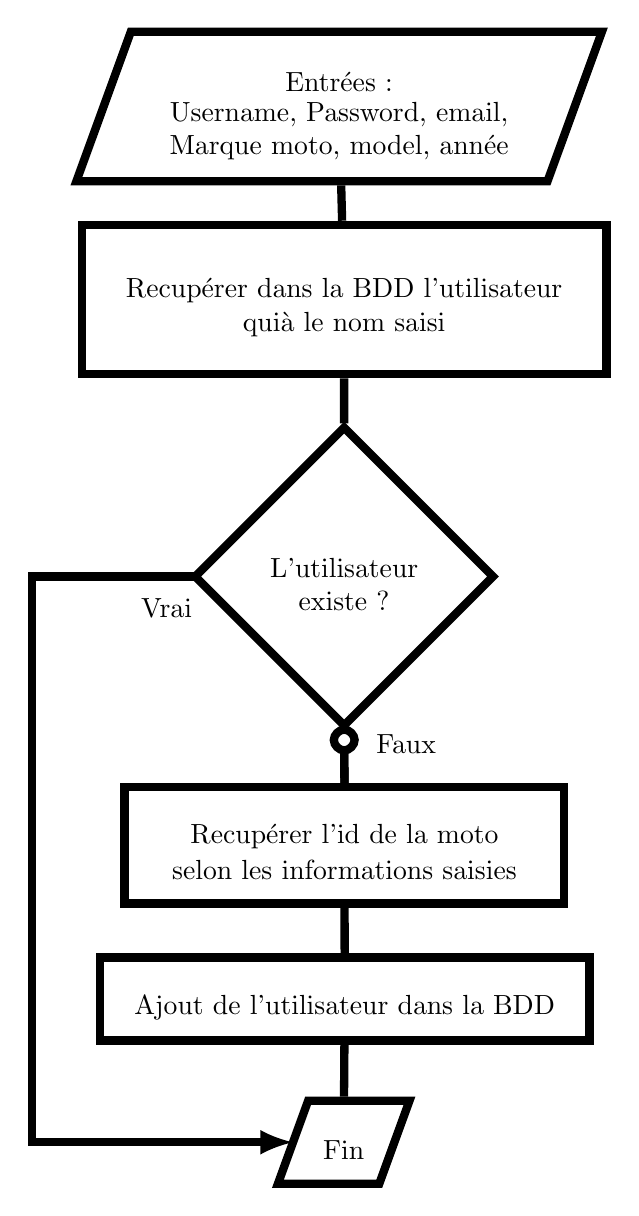
\begin{tikzpicture}
\pgftransformxscale{1.000000}
\pgftransformyscale{-1.000000}
\definecolor{dialinecolor}{rgb}{0.000000, 0.000000, 0.000000}
\pgfsetstrokecolor{dialinecolor}
\definecolor{dialinecolor}{rgb}{1.000000, 1.000000, 1.000000}
\pgfsetfillcolor{dialinecolor}
\definecolor{dialinecolor}{rgb}{1.000000, 1.000000, 1.000000}
\pgfsetfillcolor{dialinecolor}
\fill (22.383886\du,3.050000\du)--(33.732414\du,3.050000\du)--(32.422121\du,6.650000\du)--(21.073593\du,6.650000\du)--cycle;
\pgfsetlinewidth{0.200000\du}
\pgfsetdash{}{0pt}
\pgfsetdash{}{0pt}
\pgfsetmiterjoin
\definecolor{dialinecolor}{rgb}{0.000000, 0.000000, 0.000000}
\pgfsetstrokecolor{dialinecolor}
\draw (22.383886\du,3.050000\du)--(33.732414\du,3.050000\du)--(32.422121\du,6.650000\du)--(21.073593\du,6.650000\du)--cycle;
% setfont left to latex
\definecolor{dialinecolor}{rgb}{0.000000, 0.000000, 0.000000}
\pgfsetstrokecolor{dialinecolor}
\node at (27.403004\du,4.245000\du){Entrées :};
% setfont left to latex
\definecolor{dialinecolor}{rgb}{0.000000, 0.000000, 0.000000}
\pgfsetstrokecolor{dialinecolor}
\node at (27.403004\du,5.045000\du){Username, Password, email,};
% setfont left to latex
\definecolor{dialinecolor}{rgb}{0.000000, 0.000000, 0.000000}
\pgfsetstrokecolor{dialinecolor}
\node at (27.403004\du,5.845000\du){Marque moto, model, année };
\definecolor{dialinecolor}{rgb}{1.000000, 1.000000, 1.000000}
\pgfsetfillcolor{dialinecolor}
\fill (21.202248\du,7.700000\du)--(21.202248\du,11.300000\du)--(33.844748\du,11.300000\du)--(33.844748\du,7.700000\du)--cycle;
\pgfsetlinewidth{0.200000\du}
\pgfsetdash{}{0pt}
\pgfsetdash{}{0pt}
\pgfsetmiterjoin
\definecolor{dialinecolor}{rgb}{0.000000, 0.000000, 0.000000}
\pgfsetstrokecolor{dialinecolor}
\draw (21.202248\du,7.700000\du)--(21.202248\du,11.300000\du)--(33.844748\du,11.300000\du)--(33.844748\du,7.700000\du)--cycle;
% setfont left to latex
\definecolor{dialinecolor}{rgb}{0.000000, 0.000000, 0.000000}
\pgfsetstrokecolor{dialinecolor}
\node at (27.523498\du,9.295000\du){Recupérer dans la BDD l'utilisateur };
% setfont left to latex
\definecolor{dialinecolor}{rgb}{0.000000, 0.000000, 0.000000}
\pgfsetstrokecolor{dialinecolor}
\node at (27.523498\du,10.095000\du){quià le nom saisi};
\definecolor{dialinecolor}{rgb}{1.000000, 1.000000, 1.000000}
\pgfsetfillcolor{dialinecolor}
\fill (27.523312\du,12.584098\du)--(31.108107\du,16.171932\du)--(27.523312\du,19.759767\du)--(23.938517\du,16.171932\du)--cycle;
\pgfsetlinewidth{0.200000\du}
\pgfsetdash{}{0pt}
\pgfsetdash{}{0pt}
\pgfsetmiterjoin
\definecolor{dialinecolor}{rgb}{0.000000, 0.000000, 0.000000}
\pgfsetstrokecolor{dialinecolor}
\draw (27.523312\du,12.584098\du)--(31.108107\du,16.171932\du)--(27.523312\du,19.759767\du)--(23.938517\du,16.171932\du)--cycle;
% setfont left to latex
\definecolor{dialinecolor}{rgb}{0.000000, 0.000000, 0.000000}
\pgfsetstrokecolor{dialinecolor}
\node at (27.523312\du,15.966932\du){L'utilisateur};
% setfont left to latex
\definecolor{dialinecolor}{rgb}{0.000000, 0.000000, 0.000000}
\pgfsetstrokecolor{dialinecolor}
\node at (27.523312\du,16.766932\du){ existe ?};
\definecolor{dialinecolor}{rgb}{1.000000, 1.000000, 1.000000}
\pgfsetfillcolor{dialinecolor}
\fill (22.235722\du,21.250000\du)--(22.235722\du,24.050000\du)--(32.825722\du,24.050000\du)--(32.825722\du,21.250000\du)--cycle;
\pgfsetlinewidth{0.200000\du}
\pgfsetdash{}{0pt}
\pgfsetdash{}{0pt}
\pgfsetmiterjoin
\definecolor{dialinecolor}{rgb}{0.000000, 0.000000, 0.000000}
\pgfsetstrokecolor{dialinecolor}
\draw (22.235722\du,21.250000\du)--(22.235722\du,24.050000\du)--(32.825722\du,24.050000\du)--(32.825722\du,21.250000\du)--cycle;
% setfont left to latex
\definecolor{dialinecolor}{rgb}{0.000000, 0.000000, 0.000000}
\pgfsetstrokecolor{dialinecolor}
\node at (27.530722\du,22.445000\du){Recupérer l'id de la moto};
% setfont left to latex
\definecolor{dialinecolor}{rgb}{0.000000, 0.000000, 0.000000}
\pgfsetstrokecolor{dialinecolor}
\node at (27.530722\du,23.245000\du){selon les informations saisies};
\definecolor{dialinecolor}{rgb}{1.000000, 1.000000, 1.000000}
\pgfsetfillcolor{dialinecolor}
\fill (21.644197\du,25.350000\du)--(21.644197\du,27.350000\du)--(33.431697\du,27.350000\du)--(33.431697\du,25.350000\du)--cycle;
\pgfsetlinewidth{0.200000\du}
\pgfsetdash{}{0pt}
\pgfsetdash{}{0pt}
\pgfsetmiterjoin
\definecolor{dialinecolor}{rgb}{0.000000, 0.000000, 0.000000}
\pgfsetstrokecolor{dialinecolor}
\draw (21.644197\du,25.350000\du)--(21.644197\du,27.350000\du)--(33.431697\du,27.350000\du)--(33.431697\du,25.350000\du)--cycle;
% setfont left to latex
\definecolor{dialinecolor}{rgb}{0.000000, 0.000000, 0.000000}
\pgfsetstrokecolor{dialinecolor}
\node at (27.537947\du,26.545000\du){Ajout de l'utilisateur dans la BDD};
\definecolor{dialinecolor}{rgb}{1.000000, 1.000000, 1.000000}
\pgfsetfillcolor{dialinecolor}
\fill (26.656044\du,28.800000\du)--(29.097220\du,28.800000\du)--(28.369280\du,30.800000\du)--(25.928104\du,30.800000\du)--cycle;
\pgfsetlinewidth{0.200000\du}
\pgfsetdash{}{0pt}
\pgfsetdash{}{0pt}
\pgfsetmiterjoin
\definecolor{dialinecolor}{rgb}{0.000000, 0.000000, 0.000000}
\pgfsetstrokecolor{dialinecolor}
\draw (26.656044\du,28.800000\du)--(29.097220\du,28.800000\du)--(28.369280\du,30.800000\du)--(25.928104\du,30.800000\du)--cycle;
% setfont left to latex
\definecolor{dialinecolor}{rgb}{0.000000, 0.000000, 0.000000}
\pgfsetstrokecolor{dialinecolor}
\node at (27.512662\du,29.995000\du){Fin};
\pgfsetlinewidth{0.200000\du}
\pgfsetdash{}{0pt}
\pgfsetdash{}{0pt}
\pgfsetmiterjoin
\pgfsetbuttcap
{
\definecolor{dialinecolor}{rgb}{0.000000, 0.000000, 0.000000}
\pgfsetfillcolor{dialinecolor}
% was here!!!
\pgfsetarrowsend{latex}
{\pgfsetcornersarced{\pgfpoint{0.000000\du}{0.000000\du}}\definecolor{dialinecolor}{rgb}{0.000000, 0.000000, 0.000000}
\pgfsetstrokecolor{dialinecolor}
\draw (23.938517\du,16.171932\du)--(20.000000\du,16.171932\du)--(20.000000\du,29.800000\du)--(26.292074\du,29.800000\du);
}}
\pgfsetlinewidth{0.200000\du}
\pgfsetdash{}{0pt}
\pgfsetdash{}{0pt}
\pgfsetbuttcap
{
\definecolor{dialinecolor}{rgb}{0.000000, 0.000000, 0.000000}
\pgfsetfillcolor{dialinecolor}
% was here!!!
\definecolor{dialinecolor}{rgb}{0.000000, 0.000000, 0.000000}
\pgfsetstrokecolor{dialinecolor}
\draw (27.452219\du,6.749280\du)--(27.474282\du,7.600720\du);
}
\pgfsetlinewidth{0.200000\du}
\pgfsetdash{}{0pt}
\pgfsetdash{}{0pt}
\pgfsetbuttcap
{
\definecolor{dialinecolor}{rgb}{0.000000, 0.000000, 0.000000}
\pgfsetfillcolor{dialinecolor}
% was here!!!
\definecolor{dialinecolor}{rgb}{0.000000, 0.000000, 0.000000}
\pgfsetstrokecolor{dialinecolor}
\draw (27.523498\du,9.500000\du)--(27.523498\du,9.500000\du);
}
\pgfsetlinewidth{0.200000\du}
\pgfsetdash{}{0pt}
\pgfsetdash{}{0pt}
\pgfsetbuttcap
{
\definecolor{dialinecolor}{rgb}{0.000000, 0.000000, 0.000000}
\pgfsetfillcolor{dialinecolor}
% was here!!!
\definecolor{dialinecolor}{rgb}{0.000000, 0.000000, 0.000000}
\pgfsetstrokecolor{dialinecolor}
\draw (27.523445\du,11.400100\du)--(27.523415\du,12.484113\du);
}
\pgfsetlinewidth{0.200000\du}
\pgfsetdash{}{0pt}
\pgfsetdash{}{0pt}
\pgfsetbuttcap
{
\definecolor{dialinecolor}{rgb}{0.000000, 0.000000, 0.000000}
\pgfsetfillcolor{dialinecolor}
% was here!!!
\definecolor{dialinecolor}{rgb}{0.000000, 0.000000, 0.000000}
\pgfsetstrokecolor{dialinecolor}
\draw (27.533651\du,24.149963\du)--(27.535800\du,25.250659\du);
}
\pgfsetlinewidth{0.200000\du}
\pgfsetdash{}{0pt}
\pgfsetdash{}{0pt}
\pgfsetbuttcap
{
\definecolor{dialinecolor}{rgb}{0.000000, 0.000000, 0.000000}
\pgfsetfillcolor{dialinecolor}
% was here!!!
\definecolor{dialinecolor}{rgb}{0.000000, 0.000000, 0.000000}
\pgfsetstrokecolor{dialinecolor}
\draw (27.529891\du,27.449182\du)--(27.520718\du,28.700818\du);
}
% setfont left to latex
\definecolor{dialinecolor}{rgb}{0.000000, 0.000000, 0.000000}
\pgfsetstrokecolor{dialinecolor}
\node[anchor=west] at (22.310747\du,16.942492\du){Vrai};
% setfont left to latex
\definecolor{dialinecolor}{rgb}{0.000000, 0.000000, 0.000000}
\pgfsetstrokecolor{dialinecolor}
\node[anchor=west] at (27.978357\du,20.200403\du){Faux};
\pgfsetlinewidth{0.200000\du}
\pgfsetdash{}{0pt}
\pgfsetdash{}{0pt}
\pgfsetbuttcap
{
\definecolor{dialinecolor}{rgb}{0.000000, 0.000000, 0.000000}
\pgfsetfillcolor{dialinecolor}
% was here!!!
\definecolor{dialinecolor}{rgb}{0.000000, 0.000000, 0.000000}
\pgfsetstrokecolor{dialinecolor}
\draw (27.523312\du,19.759767\du)--(27.530722\du,21.250000\du);
}
\definecolor{dialinecolor}{rgb}{0.000000, 0.000000, 0.000000}
\pgfsetstrokecolor{dialinecolor}
\draw (27.526295\du,20.359759\du)--(27.530722\du,21.250000\du);
\pgfsetlinewidth{0.200000\du}
\pgfsetdash{}{0pt}
\pgfsetmiterjoin
\pgfsetbuttcap
\definecolor{dialinecolor}{rgb}{1.000000, 1.000000, 1.000000}
\pgfsetfillcolor{dialinecolor}
\pgfpathmoveto{\pgfpoint{27.523809\du}{19.859765\du}}
\pgfpathcurveto{\pgfpoint{27.648807\du}{19.859144\du}}{\pgfpoint{27.774427\du}{19.983521\du}}{\pgfpoint{27.775049\du}{20.108519\du}}
\pgfpathcurveto{\pgfpoint{27.775671\du}{20.233518\du}}{\pgfpoint{27.651294\du}{20.359138\du}}{\pgfpoint{27.526295\du}{20.359759\du}}
\pgfpathcurveto{\pgfpoint{27.401297\du}{20.360381\du}}{\pgfpoint{27.275677\du}{20.236004\du}}{\pgfpoint{27.275055\du}{20.111006\du}}
\pgfpathcurveto{\pgfpoint{27.274434\du}{19.986007\du}}{\pgfpoint{27.398810\du}{19.860387\du}}{\pgfpoint{27.523809\du}{19.859765\du}}
\pgfusepath{fill}
\definecolor{dialinecolor}{rgb}{0.000000, 0.000000, 0.000000}
\pgfsetstrokecolor{dialinecolor}
\pgfpathmoveto{\pgfpoint{27.523809\du}{19.859765\du}}
\pgfpathcurveto{\pgfpoint{27.648807\du}{19.859144\du}}{\pgfpoint{27.774427\du}{19.983521\du}}{\pgfpoint{27.775049\du}{20.108519\du}}
\pgfpathcurveto{\pgfpoint{27.775671\du}{20.233518\du}}{\pgfpoint{27.651294\du}{20.359138\du}}{\pgfpoint{27.526295\du}{20.359759\du}}
\pgfpathcurveto{\pgfpoint{27.401297\du}{20.360381\du}}{\pgfpoint{27.275677\du}{20.236004\du}}{\pgfpoint{27.275055\du}{20.111006\du}}
\pgfpathcurveto{\pgfpoint{27.274434\du}{19.986007\du}}{\pgfpoint{27.398810\du}{19.860387\du}}{\pgfpoint{27.523809\du}{19.859765\du}}
\pgfusepath{stroke}
\end{tikzpicture}
